%% ------------------------------------------------------------------------- %%
\chapter{Cronograma}
\label{cap:cronograma}

\section{Próximos passos}

A proposta deste trabalho é avaliar o uso das redes convolucionais no problema de \textit{code retrieval}. Conforme \cite{Goodfellow-et-al-2016:pratical-methodology}, o primeiro passo é definir um objetivo, um valor alvo para o modelo. No nosso caso, o objetivo é obter um resultado comparável ao modelo proposto por \cite{cambronero-deep-learning-code-search:2019}, que é o estado da arte atualmente.

O processo de treinamento de uma rede neural envolve algumas etapas. Desde o processo de tomada de decisão para uso de deep learning, coleta dos dados até a avaliação do modelo. Algumas etapas foram parcialmente concluídas durante o estudo preliminar. A figura~\ref{fig:neural-network-process-training} abaixo ilustra as etapas do processo de treinamento e o andamento através de um mapa de calor.


\begin{figure}[h]
    \centering
    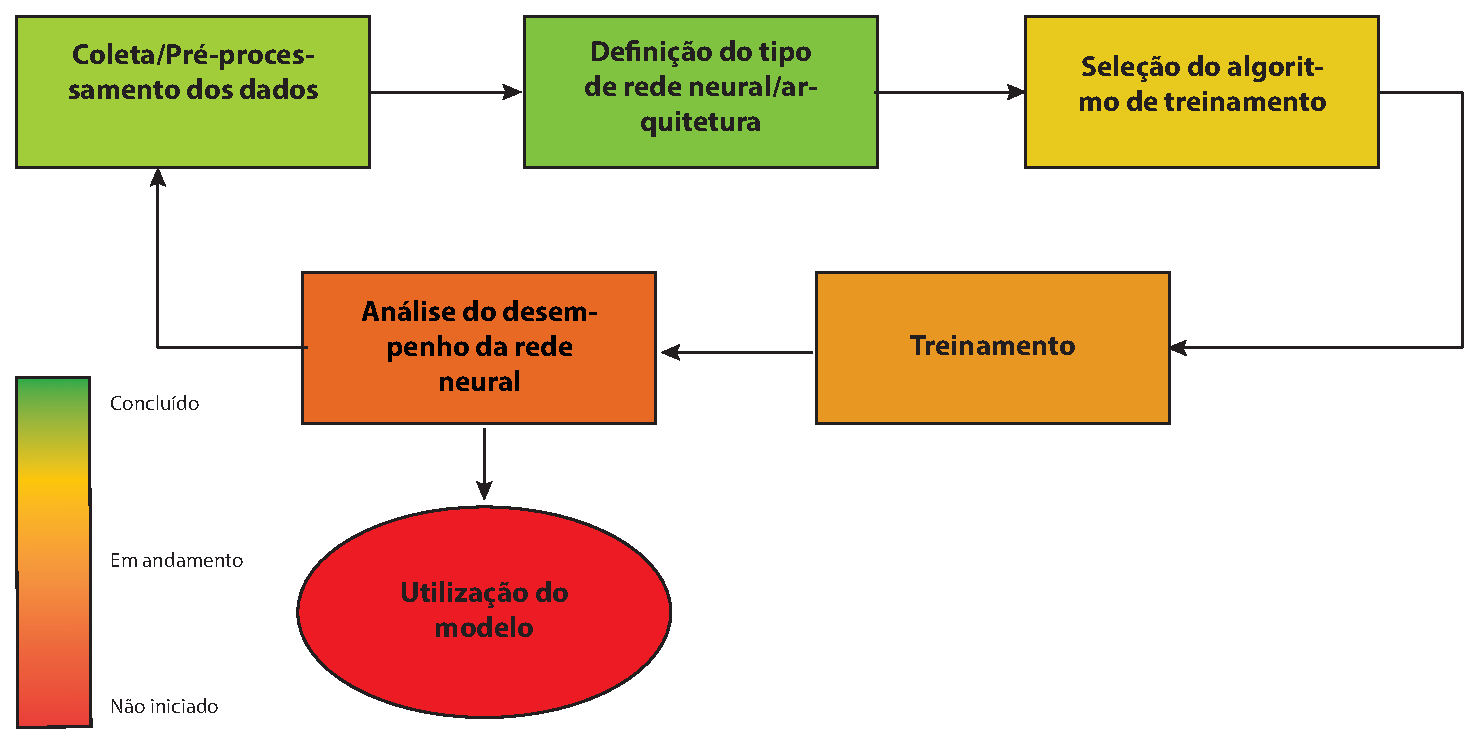
\includegraphics[width=1\textwidth]{figuras/cap-cronograma/training_process.pdf}
    \caption{Etapas do processo de treinamento de uma rede neural. As etapas de \emph{Análise do desempenho da rede neural} e \emph{Seleção dos hiper-parâmetros \& Treinamento} estão no início. Enquanto a \emph{Coleta/Pré-processamento dos dados} e \emph{Definição do tipo de rede neural/arquitetura} estão parcialmente concluídas. Figura adaptada do livro \cite{nndesign:2014:pratical-training-issues}}
    \label{fig:neural-network-process-training}
\end{figure}

\begin{longtable}{ p{10em} p{10em} p{10em} p{6em} }
%\centering
%\begin{tabular}{ p{10em} p{10em} p{10em} p{6em} }
\hline
\textbf{Etapa} & \textbf{Atividade} & \textbf{Tarefa} & \textbf{Status} \\
\hline
Coleta/Pré-processamento dos dados & Utilização dos dados coletados por \cite{yao-2018} & & Concluído  \\
\hline

Coleta/Pré-processamento dos dados & Pré-processamento dos dados & Verificar a possibilidade de quebra das palavras do código-fonte de acordo com a convençao de nomenclatura (\textit{snake case}). E analisar a possibilidade de remoção de \textit{stop words} & Parcialmente concluído  \\
\hline

Coleta/Pré-processamento dos dados & Treinamento não-supervisionado: \textit{word2vec} & Análise melhor do vetor de representação distribuída e se há necessidade de ajustes nos parâmetros de treinamento e dimensão do vetor & Parcialmente concluído  \\
\hline

Definição do tipo de rede neural/arquitetura & Dois modelos propostos: bi-LSTM com CNN e CNN & & Concluído  \\
\hline

Definição do tipo de rede neural/arquitetura & Modelos para comparação: \textit{Embedding} e o \textit{bi-modal embedding} com o mecanismo de atenção proposto por \cite{cambronero-deep-learning-code-search:2019} & & Concluído  \\
\hline

Definição do tipo de rede neural/arquitetura & Definição do objetivo: Resultado comparável ao modelo proposto por \cite{cambronero-deep-learning-code-search:2019} em um mesmo ambiente de testes e conjunto de dados & Inicialmente, buscamos um desempenho superior em pelo menos 10p.p. em relação ao modelo do \cite{cambronero-deep-learning-code-search:2019}. Dependendo do desempenho do nosso modelo, este valor alvo pode ser revisto & Parcialmente Concluído  \\
\hline

Definição do tipo de rede neural/arquitetura & Seleção dos hiper-parâmetros do modelo & Esta tarefa será feita em conjunto com o treinamento. Conforme o desempenho do modelo, ajustes nos hiper-parâmetros devem ser feitos para aumentar ou diminuir a capacidade do modelo & Em andamento  \\
\hline

 
%\end{tabular}
\caption{Relação da quantidade de dados utilizada para treinamento e avaliação dos modelos. A coluna \textbf{\# questões anotadas} refere-se a quantidade de questões anotadas manualmente para avaliação final do modelo.}
\label{table:etapas-processo-treinamento}
\end{longtable}


Coleta dos dados -> pré processamento -> treinamento -> avaliação 



Definir metrica de desempenho

Default baseline model

Selecionando hiper parâmetros

Estratégias de debug

Visualizar a pior predição (worst mistake)
















